\documentclass{article}
\usepackage{amsmath, amssymb, amsthm}
\usepackage{graphicx}
\usepackage{tikz}
\usepackage{array}

\newtheorem{theorem}{Theorem}
\newtheorem{lemma}{Lemma}

\begin{document}
	
	\title{Prüfer Code and Its Uniqueness for Trees}
	\author{Mohammad Hossein Kazemini - Mohammad Javad Abdolahi}
	\date{2025-02-25}
	\maketitle
	
	\section{Definition of Prüfer Code}
	The \textbf{Prüfer code} is a numerical sequence assigned to every labeled tree with $n$ vertices. It provides a compact representation of the tree and establishes a one‑to‑one correspondence between labeled trees and sequences of length $n-2$.
	
	\section{Algorithm to Generate Prüfer Code from a Tree}
	To generate the Prüfer code of a tree with $n$ vertices:
	\begin{enumerate}
		\item Find the smallest leaf (a vertex of degree 1).
		\item Record its neighbor in the Prüfer sequence.
		\item Remove the leaf from the tree.
		\item Repeat until only two vertices remain.
	\end{enumerate}
	
	\subsection{Example}
	Consider the following tree:
	
	\begin{center}
		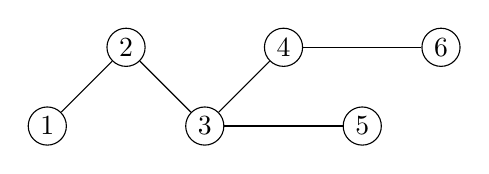
\begin{tikzpicture}[scale=1, every node/.style={circle, draw, inner sep=2pt}]
			\node (1) at (0,0) {1};
			\node (2) at (1,1) {2};
			\node (3) at (2,0) {3};
			\node (4) at (3,1) {4};
			\node (5) at (4,0) {5};
			\node (6) at (5,1) {6};
			
			\draw (1) -- (2);
			\draw (2) -- (3);
			\draw (3) -- (4);
			\draw (3) -- (5);
			\draw (4) -- (6);
		\end{tikzpicture}
	\end{center}
	
	The process of generating the Prüfer code:
	
	\begin{center}
		\begin{tabular}{|c|c|c|}
			\hline
			Step & Removed leaf & Prüfer code so far \\
			\hline
			1 & 1 (connected to 2) & 2 \\
			2 & 2 (connected to 3) & 3 \\
			3 & 5 (connected to 3) & 3 \\
			4 & 3 (connected to 4) & 4 \\
			\hline
		\end{tabular}
	\end{center}
	
	Thus the Prüfer code of this tree is:
	\[
	(2,3,3,4)
	\]
	
	\section{Algorithm to Reconstruct the Tree from a Prüfer Code}
	To reconstruct the tree from a Prüfer code:
	\begin{enumerate}
		\item Compute the degree of each vertex.
		\item Find the smallest vertex with degree 1 and connect it to the first element of the Prüfer sequence.
		\item Decrease the degree of the connected vertex, remove the leaf, and continue.
		\item When only two vertices remain, connect them.
	\end{enumerate}
	
	\subsection{Example}
	Using the Prüfer code $(2,3,3,4)$ we reconstruct the tree:
	
	\begin{center}
		\begin{tabular}{|c|c|c|}
			\hline
			Step & Edge added & Remaining Prüfer code \\
			\hline
			1 & 1 – 2 & (3,3,4) \\
			2 & 2 – 3 & (3,4) \\
			3 & 5 – 3 & (4) \\
			4 & 3 – 4 & () \\
			\hline
		\end{tabular}
	\end{center}
	
	The original tree is reconstructed (same shape as above).
	
	\section{Proof of Uniqueness}
	\begin{theorem}
		Every tree has a unique Prüfer code.
	\end{theorem}
	\begin{proof}
		The encoding process always removes the smallest leaf and records its unique neighbor. Since the smallest leaf is uniquely determined at each step, two different trees cannot produce the same Prüfer code.
	\end{proof}
	
	\begin{theorem}
		Every Prüfer code corresponds to a unique tree.
	\end{theorem}
	\begin{proof}
		In the reconstruction process, at each step the smallest vertex of degree 1 is uniquely determined and connected to the first element of the remaining code. This deterministic process yields a unique tree.
	\end{proof}
	
	\section{Conclusion}
	The Prüfer code not only provides a compact representation of a tree but also allows us to count the number of labeled trees. The number of labeled trees with $n$ vertices is:
	\[
	n^{n-2}
	\]
	which equals the number of distinct Prüfer sequences.
	
\end{document}